\section{Анализ подходов и технологий к разработке платформы
для интерактивного формирования запросов к языковым и генеративным
нейросетям}
\label{sec:analysis}
Платформы для интерактивного формирования запросов к языковым и генеративным нейросетям помогают пользователям составлять эффективные и подробные инструкции для моделей. Крупные языковые модели (Large Language Models, LLM) чувствительны к тому, как сформулирован запрос: четкость, контекст и структура запроса напрямую влияют на качество ответа. Prompt engineering – это практика улучшения запросов для получения более релевантных и точных результатов от нейросетей\cite{lakera:2025}. данном исследовании рассматриваются подходы к улучшению детализации и структуры запросов, анализируются существующие системы для генерации подсказок, обсуждаются архитектурные варианты построения таких платформ и возможные модели (NLP и ML) для автоматического улучшения запросов.
\subsection{Методы улучшения детализации и структуры запросов}
\begin{figure}[htbp]
    \centering
    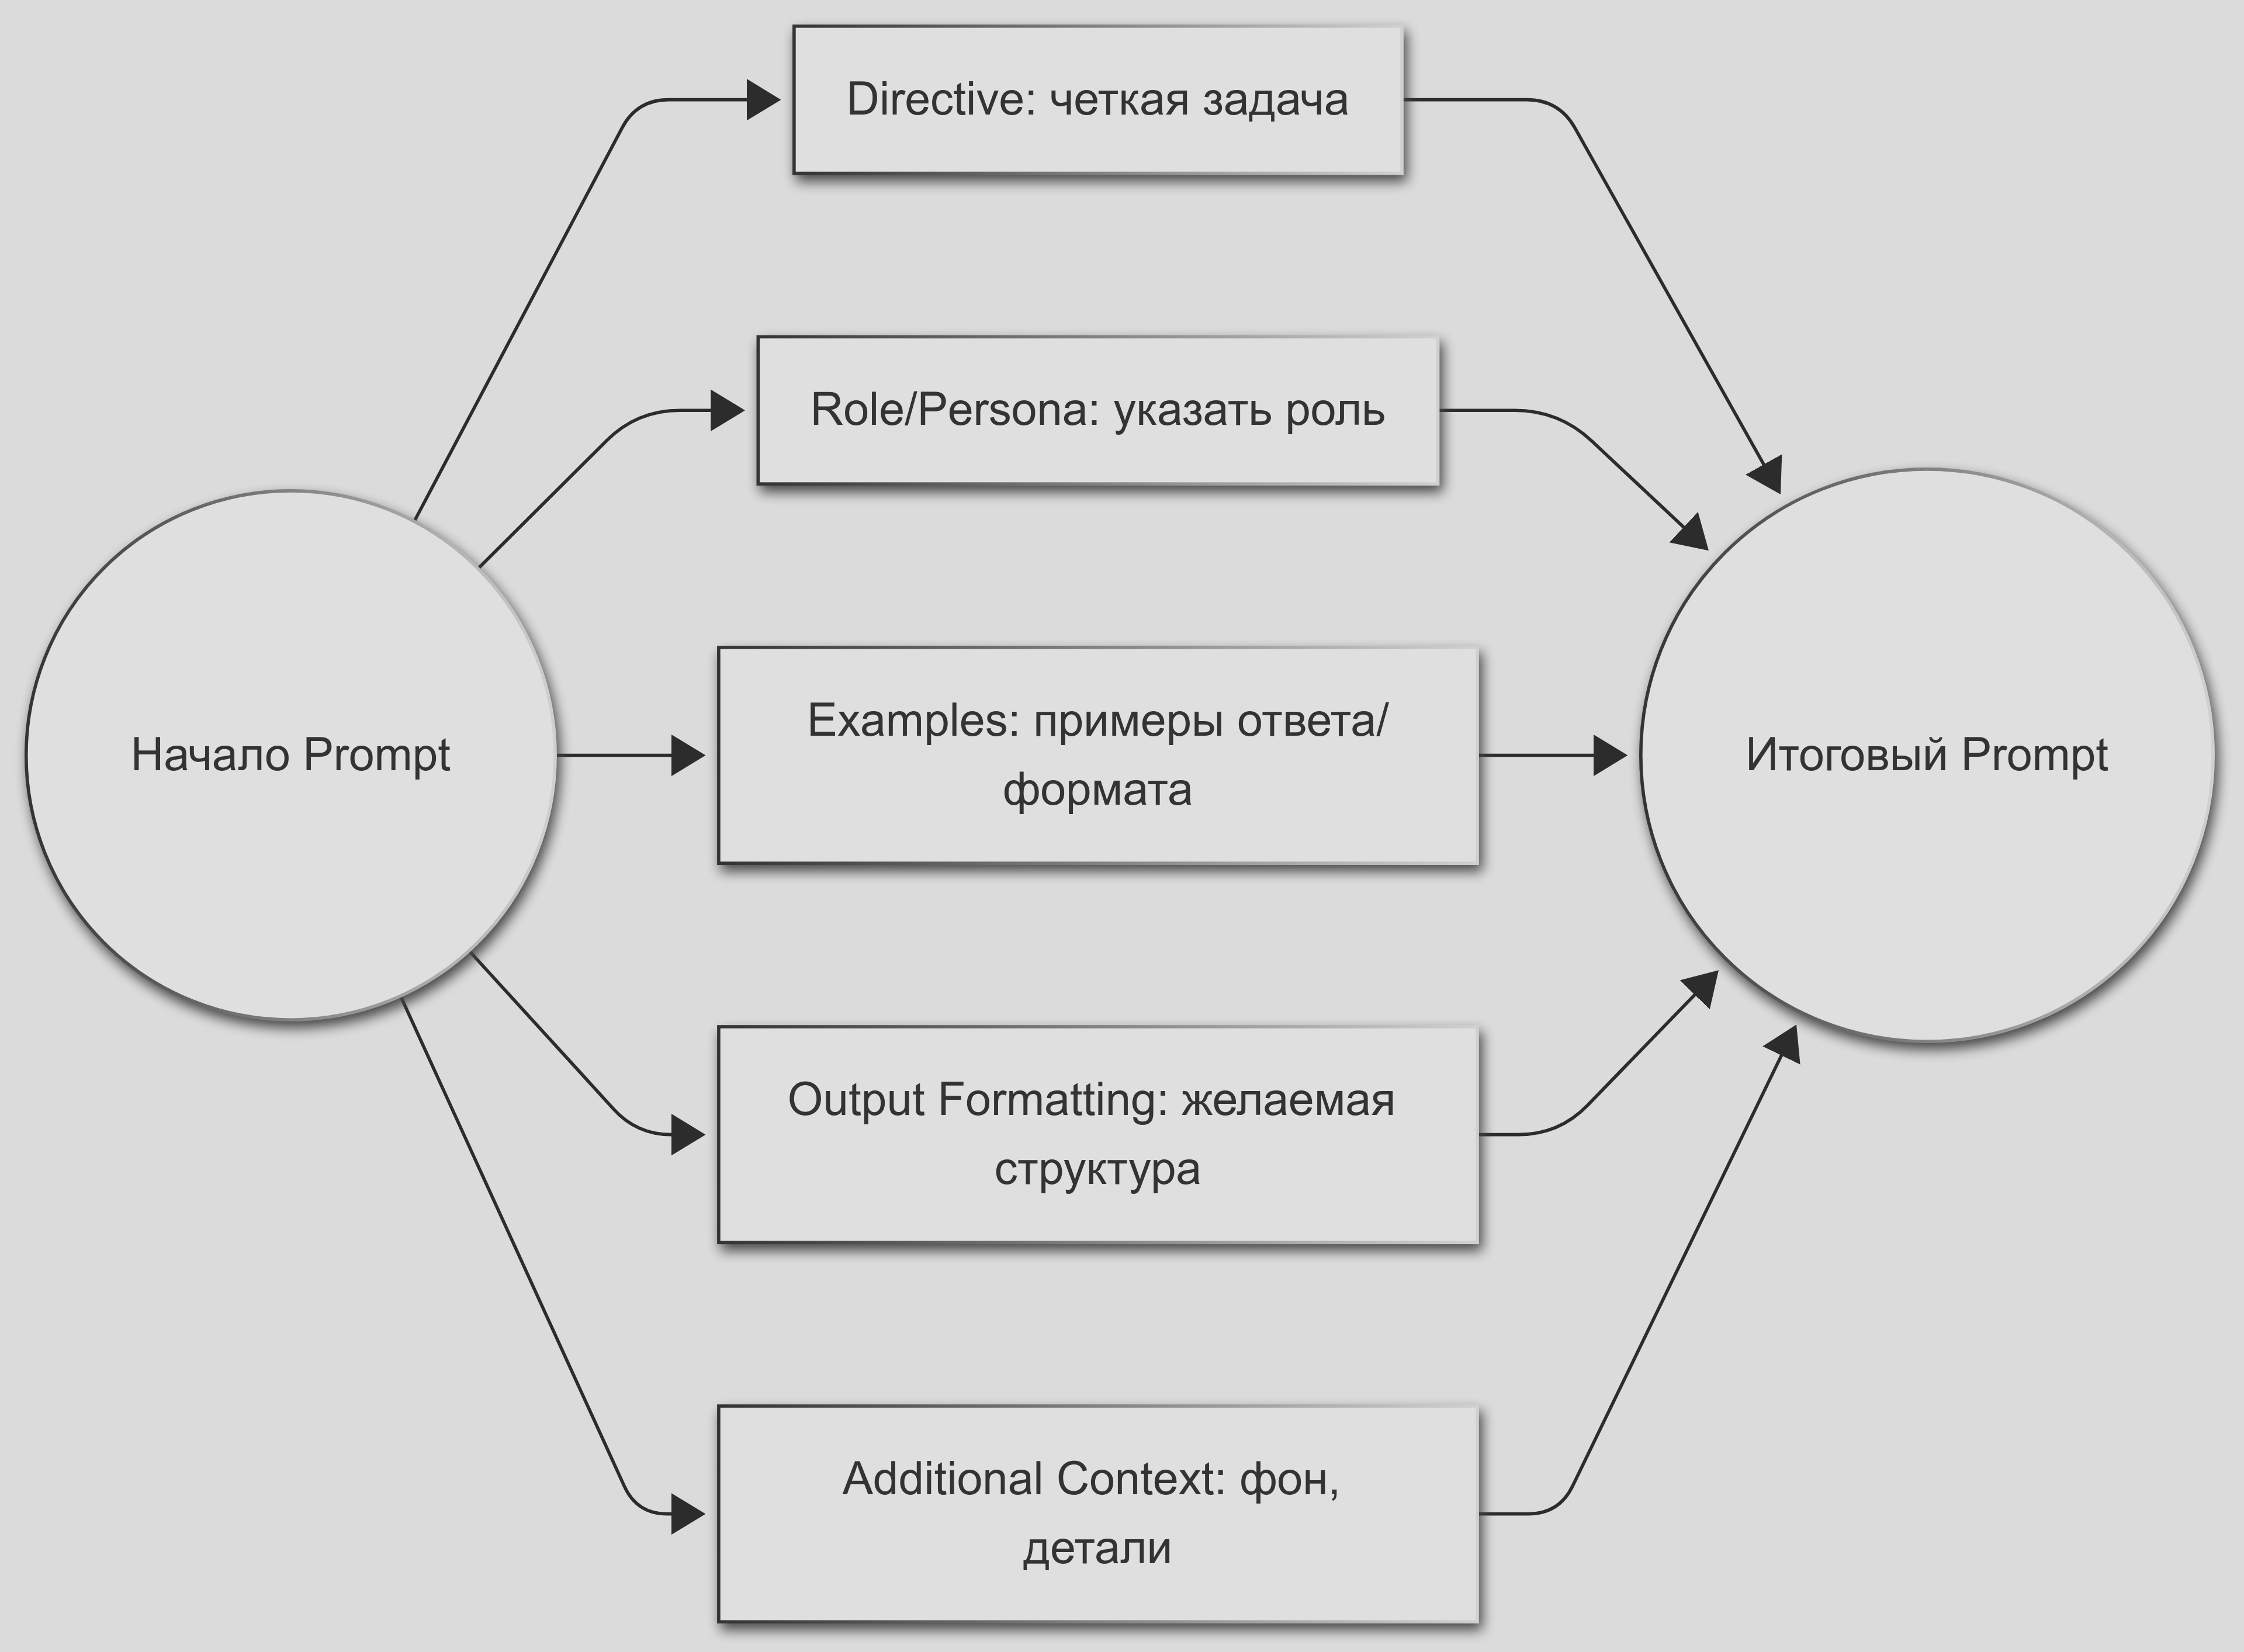
\includegraphics[width=0.8\textwidth]{picture/diploma_prompt_structure.png}
    \caption{Аспекты качественного запроса}
    \label{prompt_quality_props}
\end{figure}
Качественный запрос обычно содержит несколько ключевых элементов, обеспечивающих модели необходимый контекст\cite{learnprompt:promptstructure} они представлены на рисунке \ref{prompt_quality_props}. 
Во-первых, четкая директива (The Directive) – основная инструкция, указывающая модели, что нужно сделать.
Без ясной директивы модель может дать расплывчатый или не относящийся к делу ответ\cite{learnprompt:promptstructure}. Поэтому запрос должен содержать конкретный глагол действия и формулировать задачу напрямую (например, «составь список из пяти книг по теме...», вместо общего «расскажи что-нибудь интересное»).

Во-вторых, полезно приводить примеры (Examples) выполнения задачи, особенно для сложных или специфичных запросов. Пример(ы) в запросах демонстрируют желаемый формат или стиль ответа, помогая модели понять ожидаемый результат \cite{learnprompt:promptstructure}. Например, прежде чем попросить модель переводить предложения, можно показать один-два примера исходного текста и правильного перевода – тогда модель с большей вероятностью продолжит в заданном формате\cite{learnprompt:promptstructure}.

В-третьих, можно задать модели роль или персону (Role/Persona). Указывая, что «Ты – эксперт-историк» или «Представь себя профессиональным переводчиком», мы настраиваем тон и стиль ответа под нужный нам контекст \cite{learnprompt:promptstructure}. Такой явный контекст задаёт модели рамки: например, ответ «от лица врача» будет более формальным и содержательным в медицинской тематике. Чёткое определение роли помогает повысить релевантность и точность ответа в требуемом стиле.

Кроме того, стоит явно указывать желаемый формат вывода (Output Formatting) – например, запросить ответ в виде маркированного списка, таблицы или конкретной структуры. Наконец, полезно добавить дополнительную информацию и контекст (Additional Information): любой фон, ограничения или детали, которые могут помочь модели. Чем более конкретно очерчена задача и условия, тем более целенаправленным будет ответ модели. Интерактивные генераторы подсказок часто предлагают заполнить такие поля, как роль, цель, тон ответа, длина ответа, дополнительные детали, чтобы ничего не упустить при формулировании запроса\cite{copilotworks:promptgen}. 

Оптимизация структуры запроса. Помимо содержания, важно и то, как структурирован prompt. Рекомендуется явно разделять разные части запроса – контекст, сам вопрос, ограничения – либо визуальными разделителями, либо форматированием. Практика показывает, что использование разграничителей (делимитеров), таких как тэги XML, тройные кавычки \( \dots \) или угловые скобки для секций, повышает ясность структуры и понимание модели\cite{lakera:2025}. Например, можно оформить запрос с секциями \texttt{<context>...</context>}, \texttt{<user\_request>...</user\_request>}, \texttt{<constraints>...</constraints>}, что явно разделит вводные данные, собственно вопрос пользователя и особые требования\cite{lakera:2025}.

Хорошо структурированный ввод помогает модели не перепутать различную информацию и соблюдать заданные рамки при генерации ответа. Исследования по prompt engineering отмечают, что чёткие границы между разными типами данных в запросе значительно улучшают понимание и точность ответов модели\cite{lakera:2025}. 

Другой приём для сложных задач – это так называемый \textit{Chain-of-Thought} (цепочка мыслей). В запрос явно закладывается пошаговое рассуждение: мы просим модель сначала размышлять или вывести промежуточные шаги, прежде чем дать итоговый ответ. Такой \textit{Chain-of-Thought prompting} побуждает модель разбить сложную задачу на более простые части и решать их последовательно\cite{lakera:2025}. Исследования показывают, что без структуры модели путаются в многошаговых рассуждениях, тогда как запрос в формате «Шаг 1: \dots; Шаг 2: \dots; Вывод: \dots» даёт более логичные результаты\cite{lakera:2025}. Например, для задачи решения головоломки или математической задачи, можно явно попросить: «Реши задачу пошагово: сначала проанализируй условия, затем вычисли промежуточные значения, и в конце дай ответ». Такая структура заставляет нейросеть имитировать процесс размышления человека и выдавать более обоснованные ответы.

Уточнение и детализация. Один из принципов хорошего промпта – максимальная конкретность. Чем конкретнее и однозначнее сформулирован запрос, тем меньше шансов на размытый ответ. Практические советы включают: задавать конкретные вопросы, избегать жаргона и двусмысленностей, явно прописывать, что именно нужно на выходе\cite{lakera:2025}. Например, вместо расплывчатого «Расскажи про экономику», лучше спросить: «Дай краткий обзор современной экономики США, упомянув ВВП, уровень безработицы и основные вызовы, в \(2\)–\(3\) абзацах». Здесь чётко указана тема, аспекты, которые надо осветить, и даже желаемый объём ответа. Такой подход задаёт модели понятную задачу и формат ответа\cite{copilotworks:promptgen}.

Если требуется определённый стиль или тон, стоит это явно оговорить. Например: «Ответь дружелюбным тоном и простыми словами, понятными ребёнку \(10\) лет». Или: «Предоставь ответ формально, в академическом стиле, с цитированием источников». Эти уточнения направляют модель на нужный стиль изложения. В интерактивных генераторах подсказок подобные параметры часто выносятся как отдельные настройки \((\text{tone/style}, \text{reading level})\), чтобы пользователь не забыл их указать\cite{copilotworks:promptgen}.

Работа с длинными запросами и контекстом. Отдельная задача – как эффективно обрабатывать очень объёмные вводы или контекст. Современные LLM имеют ограничение на размер контекста (количество токенов), поэтому при превышении лимитов приходится искать обходные пути. Один из подходов – разбиение длинного ввода на части. Если у нас длинный документ, который нужно проанализировать, можно разбить его на несколько секций и отправлять модели последовательно, объединяя затем результаты. Разработчики отмечают, что в таком случае полезно между вызовами модели передавать краткие резюме предыдущих частей, чтобы сохранять контекст \cite{openai:longprompts}. Проще говоря, можно организовать итеративное суммирование: сначала модель резюмирует часть текста, затем этот резюме включается при обработке следующей части и так далее.

В ответе OpenAI сообщества отмечено: «Нужно разбить документ на секции и объединить полученные резюме. Если предыдущий контекст важен для последующих секций, попробуйте добавлять сокращённый контекст (например, заголовки или краткие выводы предыдущих секций) в новый запрос» \cite{openai:longprompts}. Такой подход позволяет обойти ограничение по токенам, жертвуя деталями, но сохраняя ключевую информацию.


Когда используется длинный контекст, есть и другой неожиданный трюк. Документация Anthropic (модель Claude) рекомендует размещать объёмные данные в начале prompt’а, а сам вопрос – ближе к концу \cite{willison:longcontext}. В тестах с моделью Claude было показано, что если длинный текст (~20k+ токенов) поместить перед инструкциями и вопросом, качество ответа заметно возрастает (в некоторых случаях на 30\% для сложных мультидокументных запросов) \cite{willison:longcontext}. Иными словами, модель лучше усваивает длинный контекст, если он дан сначала, а уже затем – конкретный запрос пользователя. Этот приём улучшает точность ответа, особенно когда нужно учесть сразу несколько больших фрагментов информации. Помимо порядка, Anthropic предлагает использовать специальные разметки, например, заключать важные цитаты из контекста в теги <quotes> и просить модель опираться именно на эти цитаты при ответе \cite{willison:longcontext}. Такой структурированный подход помогает модели сфокусировать внимание на релевантной информации даже при очень большом объёме данных. Наконец, улучшение промпта – это зачастую итеративный процесс. Рекомендуется протестировать запрос, посмотреть на ответ модели и при необходимости уточнить или переформулировать prompt. 90\% успешного prompt engineering – это эксперименты и доработки, и лишь 10\% – само изначальное написание промпта \cite{reddit:prompteng}. Можно применить рефлексию модели: например, попросить модель сначала проверить свой ответ на соответствие запросу или сгенерировать несколько вариантов ответа и выбрать наиболее консистентный. Такой приём называется self-consistency: модель генерирует несколько решений и затем путем сравнения выбирается наиболее частый или подходящий – это повышает надёжность результата при сложных вопросах. Также модель можно попросить объяснить, почему её ответ правильный, или найти ошибки – это помогает в критических задачах снизить количество фактических ошибок\cite{lakera:2025}. Эти техники относятся уже к продвинутым стратегиям (reflective prompting), где модель используется не только для выдачи ответа, но и для самопроверки или улучшения своего же вывода\cite{restack:advprompt}. Подводя итог, чтобы получить от нейросети детальный и точный ответ, нужно максимально конкретизировать запрос, структурировать его на понятные части (роль, задача, формат ответа, контекст, примеры) и при необходимости разбивать сложные задания на последовательные этапы. Внимательное отношение к формулировке prompt способно значительно повысить качество результатов модели\cite{lakera:2025}.
Ниже рассмотрим, как эти принципы реализованы в существующих инструментах и платформах для генерации и оптимизации запросов.
\subsection{Обзор существующих систем для генерации запросов} С ростом популярности LLM появилось множество инструментов, помогающих пользователям создавать или улучшать запросы. Рассмотрим несколько систем, их возможности, преимущества и ограничения:
\begin{enumerate}[label=\arabic*]
\item Prompt Generator for ChatGPT (CopilotWorks) – веб-инструмент для быстрого составления продуманных запросов к ChatGPT и аналогичным моделям. Пользователь заполняет готовые поля: выбирает роль (эксперт, учитель, переводчик и т.д.), формулирует цель запроса, задаёт желаемый тон или формат ответа (например, совет, объяснение, краткое резюме), ограничивает объём ответа (количество абзацев или слов) и добавляет детали или контекст\cite{copilotworks:promptgen}.  На основе этих параметров генератор собирает готовый текст prompt’а, который можно скопировать и отправить в ChatGPT\cite{copilotworks:promptgen}. Инструмент фактически реализует лучшие практики создания запросов – например, предлагает указать роль модели и чётко сформулировать цель, добавлять контекст для детализации\cite{copilotworks:promptgen}. Преимущества: простота и скорость – даже неопытный пользователь за несколько кликов получит структурированный запрос. Благодаря выпадающим спискам и подсказкам снижается вероятность забыть важный параметр (тон, формат и проч.). Такой подход обеспечивает четкость и полноту промпта, что повышает качество ответа модели. Недостатки: шаблонность – система опирается на предустановленные категории ролей, тонов и т.д., что может ограничивать гибкость. Если задача нестандартна и выходит за рамки предусмотренных опций, пользователю придётся вручную дорабатывать сгенерированный prompt. Кроме того, генератор сам по себе не гарантирует идеальный результат – он лишь структурирует запрос, но не использует ИИ для его оптимизации. Тем не менее, как отправная точка для prompt engineering этот инструмент очень полезен.

\item AISEO Prompt Enhancer – автоматизированный инструмент улучшения запросов, доступный как плагин для ChatGPT. Он был разработан компанией AISEO (известной по SEO-инструментам) и позволяет автоматически перефразировать и обогащать введённый пользователем prompt. Активируется плагин ключевым словом: если начать запрос со слова “AISEO:”, подключается модуль, который перепишет последующий текст запроса более эффективным образом \cite{restack:advprompt}, \cite{whatplugin:promptenhancer}. По сути, AISEO Prompt Enhancer выступает как надстройка над ChatGPT: пользователь набрасывает черновой запрос, а плагин трансформирует его в оптимизированный, «отполированный» запрос, предназначенный для получения наилучшего ответа от модели. Преимущества: удобство – не нужно вручную вспоминать правила хорошего промпта, достаточно в свободной форме описать, что требуется, а плагин сам отформатирует и уточнит запрос. Это снижает порог входа для новых пользователей, незнакомых с тонкостями составления вопросов к ИИ\cite{whatplugin:promptenhancer}. Улучшенные запросы получаются более подробными и релевантными задаче, за счёт чего повышается качество диалога с ChatGPT. Недостатки: плагин доступен только в платной версии ChatGPT с поддержкой плагинов, что ограничивает его аудиторию. Кроме того, универсальность – плагин не обучен под конкретную доменную область, он улучшает формулировку общим образом, поэтому при очень специализированных запросах результат может быть неидеальным. Также есть ограниченная прозрачность: пользователь видит только финальный изменённый запрос, но не всегда понятно, какие правки внёс инструмент (может затруднить обучение пользователя самостоятельному составлению prompt’ов). Тем не менее, AISEO Prompt Enhancer – эффективный способ «доверить AI улучшение запросов для AI», что особенно полезно для быстрого создания запросов.
\begin{figure}[htbp]
    \centering
    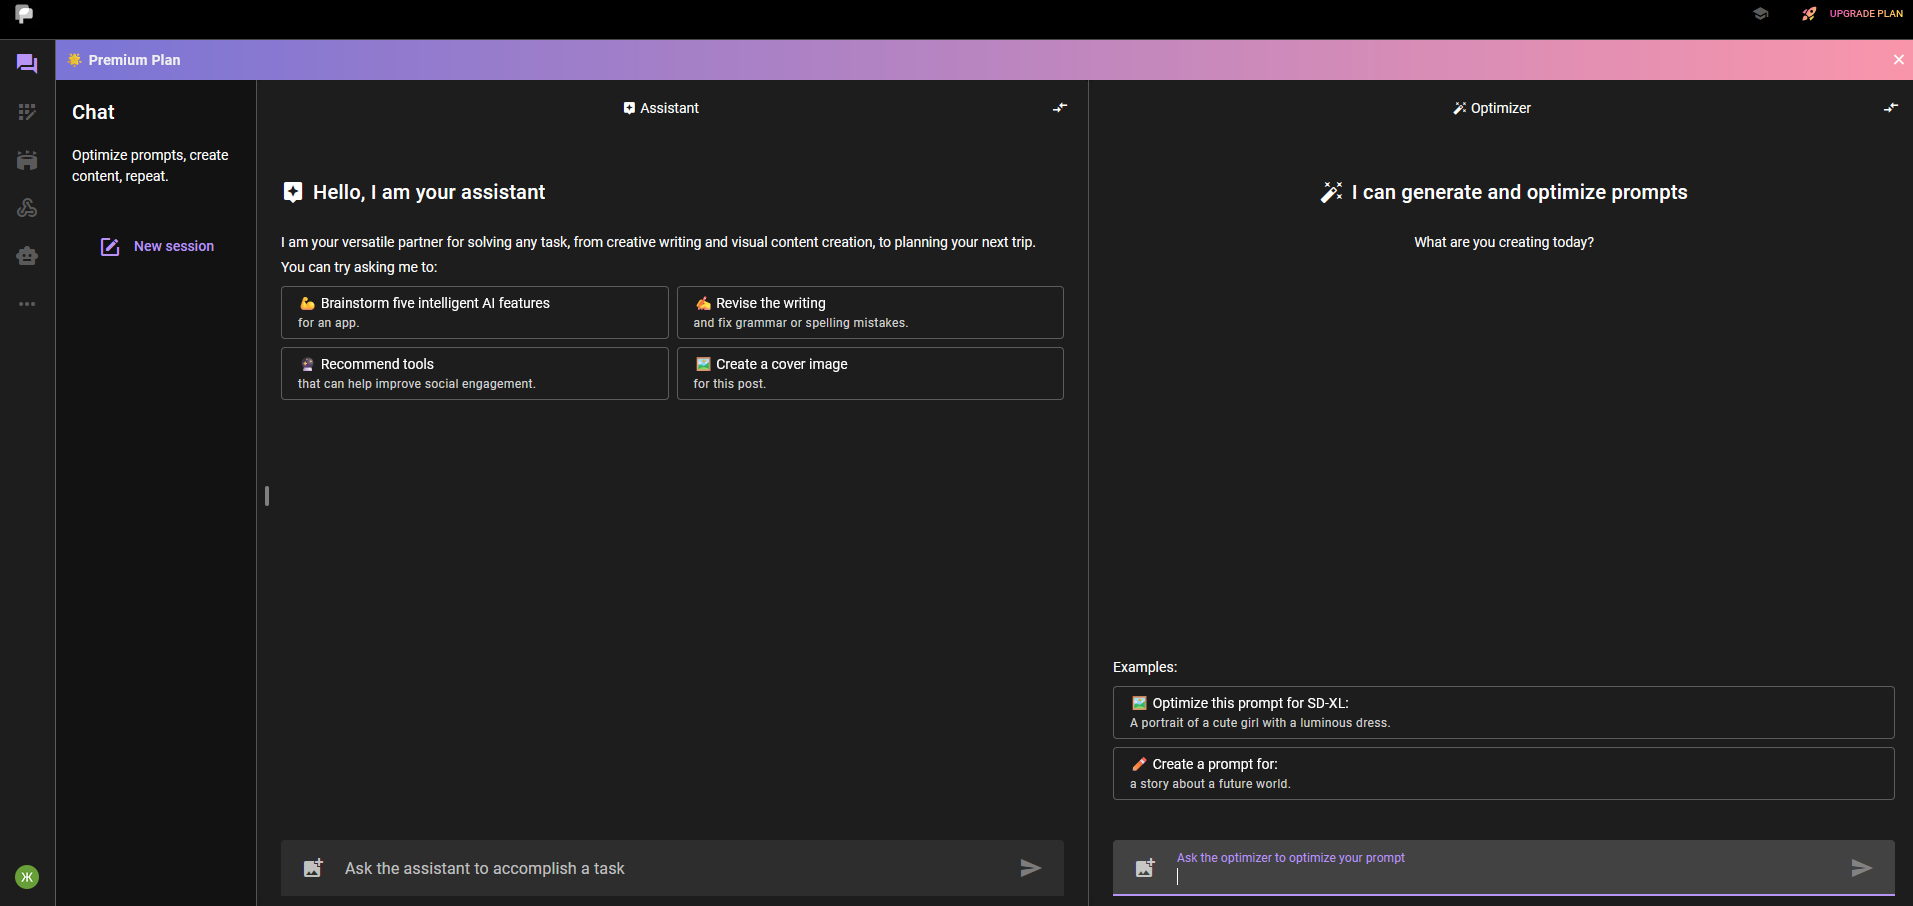
\includegraphics[width=0.8\textwidth]{picture/prompt-perfect.png}
    \caption{Веб интерфейс PromptPerfect}
    \label{prompt_perfect}
\end{figure}
\item  PromptPerfect – мощный AI-инструмент для автоматической оптимизации текстовых и визуальных запросов под различные модели. Он позиционируется как «всё-в-одном» генератор и оптимизатор промптов, поддерживающий популярные LLM (GPT-3.5/4, Claude) и генеративные модели изображений (Midjourney, DALL-E и др.) \cite{dhruvirzala:promptperfect}.Пользователь вводит исходный (сырой) запрос, выбирает целевую модель – а PromptPerfect генерирует улучшенный вариант, часто более подробный и точный. Как отмечается в обзоре, этот сервис «превращает сырые английские предложения в промпты, от которых LLM краснеют», то есть существенно обогащает и уточняет их.  Преимущества: PromptPerfect использует продвинутые техники prompt engineering под капотом. Он может автоматически добавить недостающие детали, уточнить контекст, перевести запрос на другой язык и т.п. \cite{dhruvirzala:promptperfect}. Отличительной чертой является поддержка мультиязычных промптов – инструмент способен принимать запросы на разных языках и выдавать оптимизированный prompt также на любом из поддерживаемых языков. Также сервис предлагает дополнительные функции: few-shot prompting (автоматически подставляет примеры в запрос), reverse prompt engineering для изображений (по загруженной картинке пытается сгенерировать текстовый prompt, который мог бы её описать), а также сравнение результатов разных моделей для одного и того же запроса. Наконец, у PromptPerfect есть веб-интерфейс представленный на рисунке \cite{dhruvirzala:promptperfect}. и API, что позволяет интегрировать его в рабочие процессы. Недостатки: отмечают не самую удобную UI\cite{dhruvirzala:promptperfect}. – освоить все возможности может быть непросто из-за обилия настроек (крутая кривая обучения для новичков). Кроме того, хотя базовый тариф бесплатный, для активного профессионального использования может потребоваться подписка (платный план). Ещё один нюанс – автоматическая оптимизация не всегда попадает точно в потребности пользователя, иногда может «переформулировать слишком сильно», изменив оттенки смысла. Тем не менее, выигрыш в качестве часто ощутим: инструмент действительно «добавляет детализации, повышая качество выходов ИИ»\cite{dhruvirzala:promptperfect}. В тестовом обзоре PromptPerfect получил высокие оценки за функциональность (4.7/5) и производительность (4/5), при общем рейтинге ~3.9/5 – снижают впечатление лишь нюансы интерфейса и поддержки. Это один из самых продвинутых на сегодня оптимизаторов prompt’ов, позволяющий быстро улучшать запросы для разных моделей. 
\begin{figure}[htbp]
    \centering
    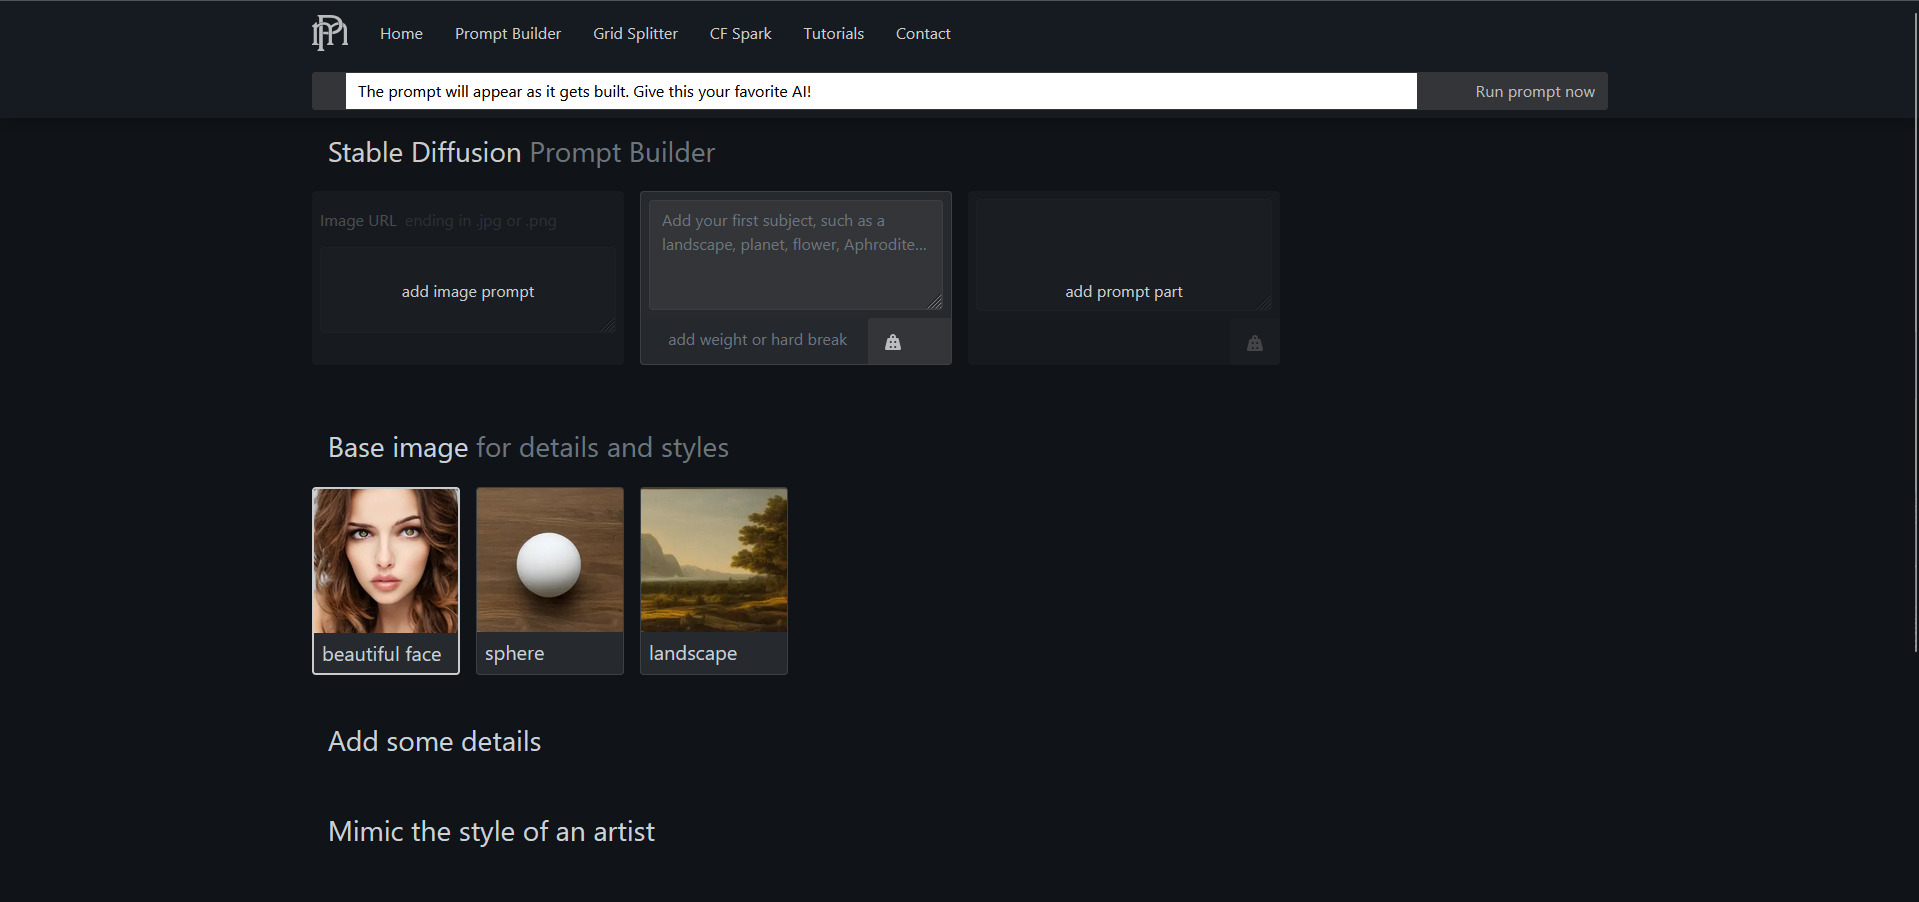
\includegraphics[width=0.8\textwidth]{picture/prompt-mania.png}
    \caption{Веб интерфейс PromptMania}
    \label{prompt_mania}
\end{figure}
\item Midjourney Prompt Generators – отдельная категория инструментов, помогающих генерировать описания для нейросетей, создающих изображения (в частности, Midjourney). Визуальные генеративные модели очень чувствительны к нюансам prompt’а: нужный стиль, детальность описания, перечисление художественных приемов. Сформулировать такой запрос сложно, поэтому появились prompt builders – интерактивные онлайн-формы, где пользователь выбирает настройки, а на выходе получает готовую строку для Midjourney\cite{promptomania:midjourney}. Пример – PromptoMANIA, бесплатный конструктор промптов для Midjourney и Stable Diffusion. . Интерфейс предлагает многочисленные опции представленные на рисунке \ref{prompt_mania}: тип сцены, художественный стиль (живопись маслом, фотореализм, акварель и т.д.), имя художника или референс (например, «в стиле Ван Гога»), параметры съемки (ракурс, объектив), качество и аспекты изображения. Преимущества: такие генераторы позволяют пользователю, не знакомому с терминологией и «секретными словами» Midjourney, легко подобрать эффектные описания. Они обычно имеют списки популярных ключевых слов: стили, жанры, освещение, цветовые схемы – которые можно комбинировать. Это гарантирует, что запрос будет содержать слова, понятные модели, и задействует известные стилистические паттерны. В результате картинки получаются более соответствующими замыслу. Кроме того, многие генераторы (PromptoMANIA, PromptHero и др.) обновляются под новые версии Midjourney\cite{promptomania:midjourney},\cite{howtoleverageai:midjourney}. учитывая лучшие практики для последней модели. Недостатки: основной минус – ограниченная креативность, поскольку пользователь выбирает из предложенных вариантов. Не все задумки может выразить готовый интерфейс, иногда требуется вручную дописать специфические детали. Также перегруженность опциями может сбивать с толку новичков – десятки выпадающих списков с художественными стилями способны запутать. Некоторые инструменты генерируют очень длинные промпты со множеством тегов – это не всегда лучше, иногда лишние теги могут внести шум. Тем не менее, для старта в работе с Midjourney они незаменимы: снижают порог входа и учат, какие слова влияют на результат. Отдельно стоит упомянуть генераторы, которые сами используют ИИ: например, сервис HowToLeverageAI предлагает сгенерировать 10 уникальных стилей одним кликом, комбинируя случайные варианты стиля для вдохновения.  Это помогает, когда хочется экспериментировать с разными художественными направлениями.

\item Stable Diffusion Prompt Generators – аналогично предыдущему, но ориентированы на модели Stable Diffusion. Поскольку SD – открытая модель, экосистема генераторов разнообразна: от простых веб-форм до открытого кода. Например, Neural Frames Stable Diffusion Prompt Generator предоставляет поле ввода для описания идеи и затем автоматически дополняет его, улучшая и уточняя для лучшего результата\cite{neuralframes:sdprompt}.  Заявлено, что он использует NLP-алгоритмы для подбора ключевых слов по введённому описанию  – то есть пользователь пишет простое описание («горный пейзаж на закате»), а система добавляет детали («HDR, 4K, dramatic lighting, by Greg Rutkowski, trending on ArtStation...» и т.п.)\cite{feedough:sdprompt}. Преимущества: экономит время и знания – не нужно самому перебирать сотни тегов, ИИ подскажет, какие ключевые слова усилят изображение. Кроме того, такие генераторы могут обучаться на больших массивах существующих промптов. В частности, открыт репозиторий модели, дообученной на 74 тысячах текстовых описаний для Stable Diffusion\cite{ollama:sdprompt}. Эта модель способна превратить краткий запрос пользователя в развернутый prompt, оптимизированный для SD\cite{ollama:sdprompt}. Такие подходы, подкрепленные данными, зачастую генерируют промпты не хуже экспертов: учитываются популярные стили, корректно расставляются весы важности слов (например, скобками или символом : в SD). Недостатки: автоматические улучшители для SD могут, подобно телефонной игре, искажать исходный замысел. Пользователь рискует получить красивый, но уже не тот кадр, что он хотел, если полностью полагается на генератор. Поэтому часто советуют использовать их как подсказку: сгенерированный prompt – основа, которую можно затем вручную отредактировать. Кроме того, некоторые инструменты (как Neural Frames) работают онлайн, и качество генерации ключевых слов может варьироваться. Однако, даже частичное дополнение запроса правильными стилевыми тегами сильно повышает качество итогового изображения\cite{feedough:sdprompt}. В целом, генераторы промптов для Stable Diffusion демократизируют использование этой сложной модели, позволяя получать красочные результаты без глубокого погружения в сообщество художников AI.

\item OctiAI Prompt Generator – относительно новая платформа (позиционируется как инструмент 2025 года), использующая комбинацию автозаполнения и ИИ для создания «идеальных промптов». OctiAI интересен своим подходом: он интерактивно задает уточняющие вопросы о вашем запросе и может автоматически заполнять ответы на них, опираясь на уже введённые данные\cite{octiai:2025}. Фактически, это полуавтоматический ассистент: пользователь описывает свой wish (желание/идею) в общем виде, далее OctiAI может сам сформулировать наводящие вопросы и сам же на них ответить, уточняя детали проекта. Сообщается, что после нескольких нажатий Enter пользователь получает персонализированный prompt, на «90\% точно отражающий его задумку», сгенерированный буквально за секунды\cite{octiai:2025}. Преимущества: OctiAI реализует принцип диалога при создании запроса – как опытный инженер по запросам, он расспрашивает о подробностях (а при авто-режиме сам логически додумывает их). Это экономит время: по сути, ИИ экстраполирует из начального замысла полный подробный сценарий. В примерах на сайте показано, как из краткой фразы «Хочу создать видео-шаблон для рекламы моего AI-приложения в TikTok» OctiAI генерирует развернутый промпт с учетом всех особенностей платформы (динамичный темп, визуальные hooks, упоминание трендов, призыв к действию и т.д.)\cite{octiai:2025}. То есть он добавляет экспертные знания о домене (TikTok-маркетинг) прямо в запрос. Для пользователя, не обладающего такими сведениями, это огромный плюс: результат – словно консультация специалиста. Недостатки: пока о нем известно не слишком много; очевидно, для такой глубокой работы OctiAI сам опирается на мощные языковые модели (возможно GPT-4), что может означать платный доступ или ограничения. Кроме того, автоматическое «додумывание» деталей за пользователя – палка о двух концах: если предположения ИИ ошибочны, итоговый prompt может увести не туда. Система заявляет 90\% точности, но 10\% расхождения могут быть критичными, особенно в творческих задачах. И, конечно, как и другие коммерческие сервисы, OctiAI – закрытая платформа, где не полностью ясно, как генерируется результат. Тем не менее, подход с автозаполнением и диалоговым уточнением представляет интересное направление: интерактивное соавторство с ИИ при создании промпта.
\end{enumerate}

Помимо перечисленных, существуют и другие решения. Например, популярное расширение AIPRM для браузера предоставляет библиотеку готовых промпт-шаблонов для ChatGPT на все случаи жизни – от маркетинга до программирования. Оно позволяет в один клик подставить сложный многошаговый запрос с переменными, экономя время. Также сообщества вроде FlowGPT обмениваются успешными промптами. Однако эти варианты меньше про автоматическую генерацию, а скорее про шаблоны и обмен опытом. В контексте же интерактивных платформ, перечисленные 5–6 систем демонстрируют разнообразные подходы: от простых форм для структурирования (Prompt Generator), через плагины и оптимизаторы на базе ИИ (AISEO, PromptPerfect), до специализированных визуальных конструкторов (для Midjourney/SD) и гибридных ассистентов (OctiAI). Каждый инструмент имеет свои сильные стороны – либо простоту, либо интеллектуальность, либо узкую заточку под конкретную модель – а пользователю и разработчику платформы важно понимать эти особенности при выборе решения.
\subsection{Архитектурные варианты платформы}
\begin{figure}[htbp]
    \centering
    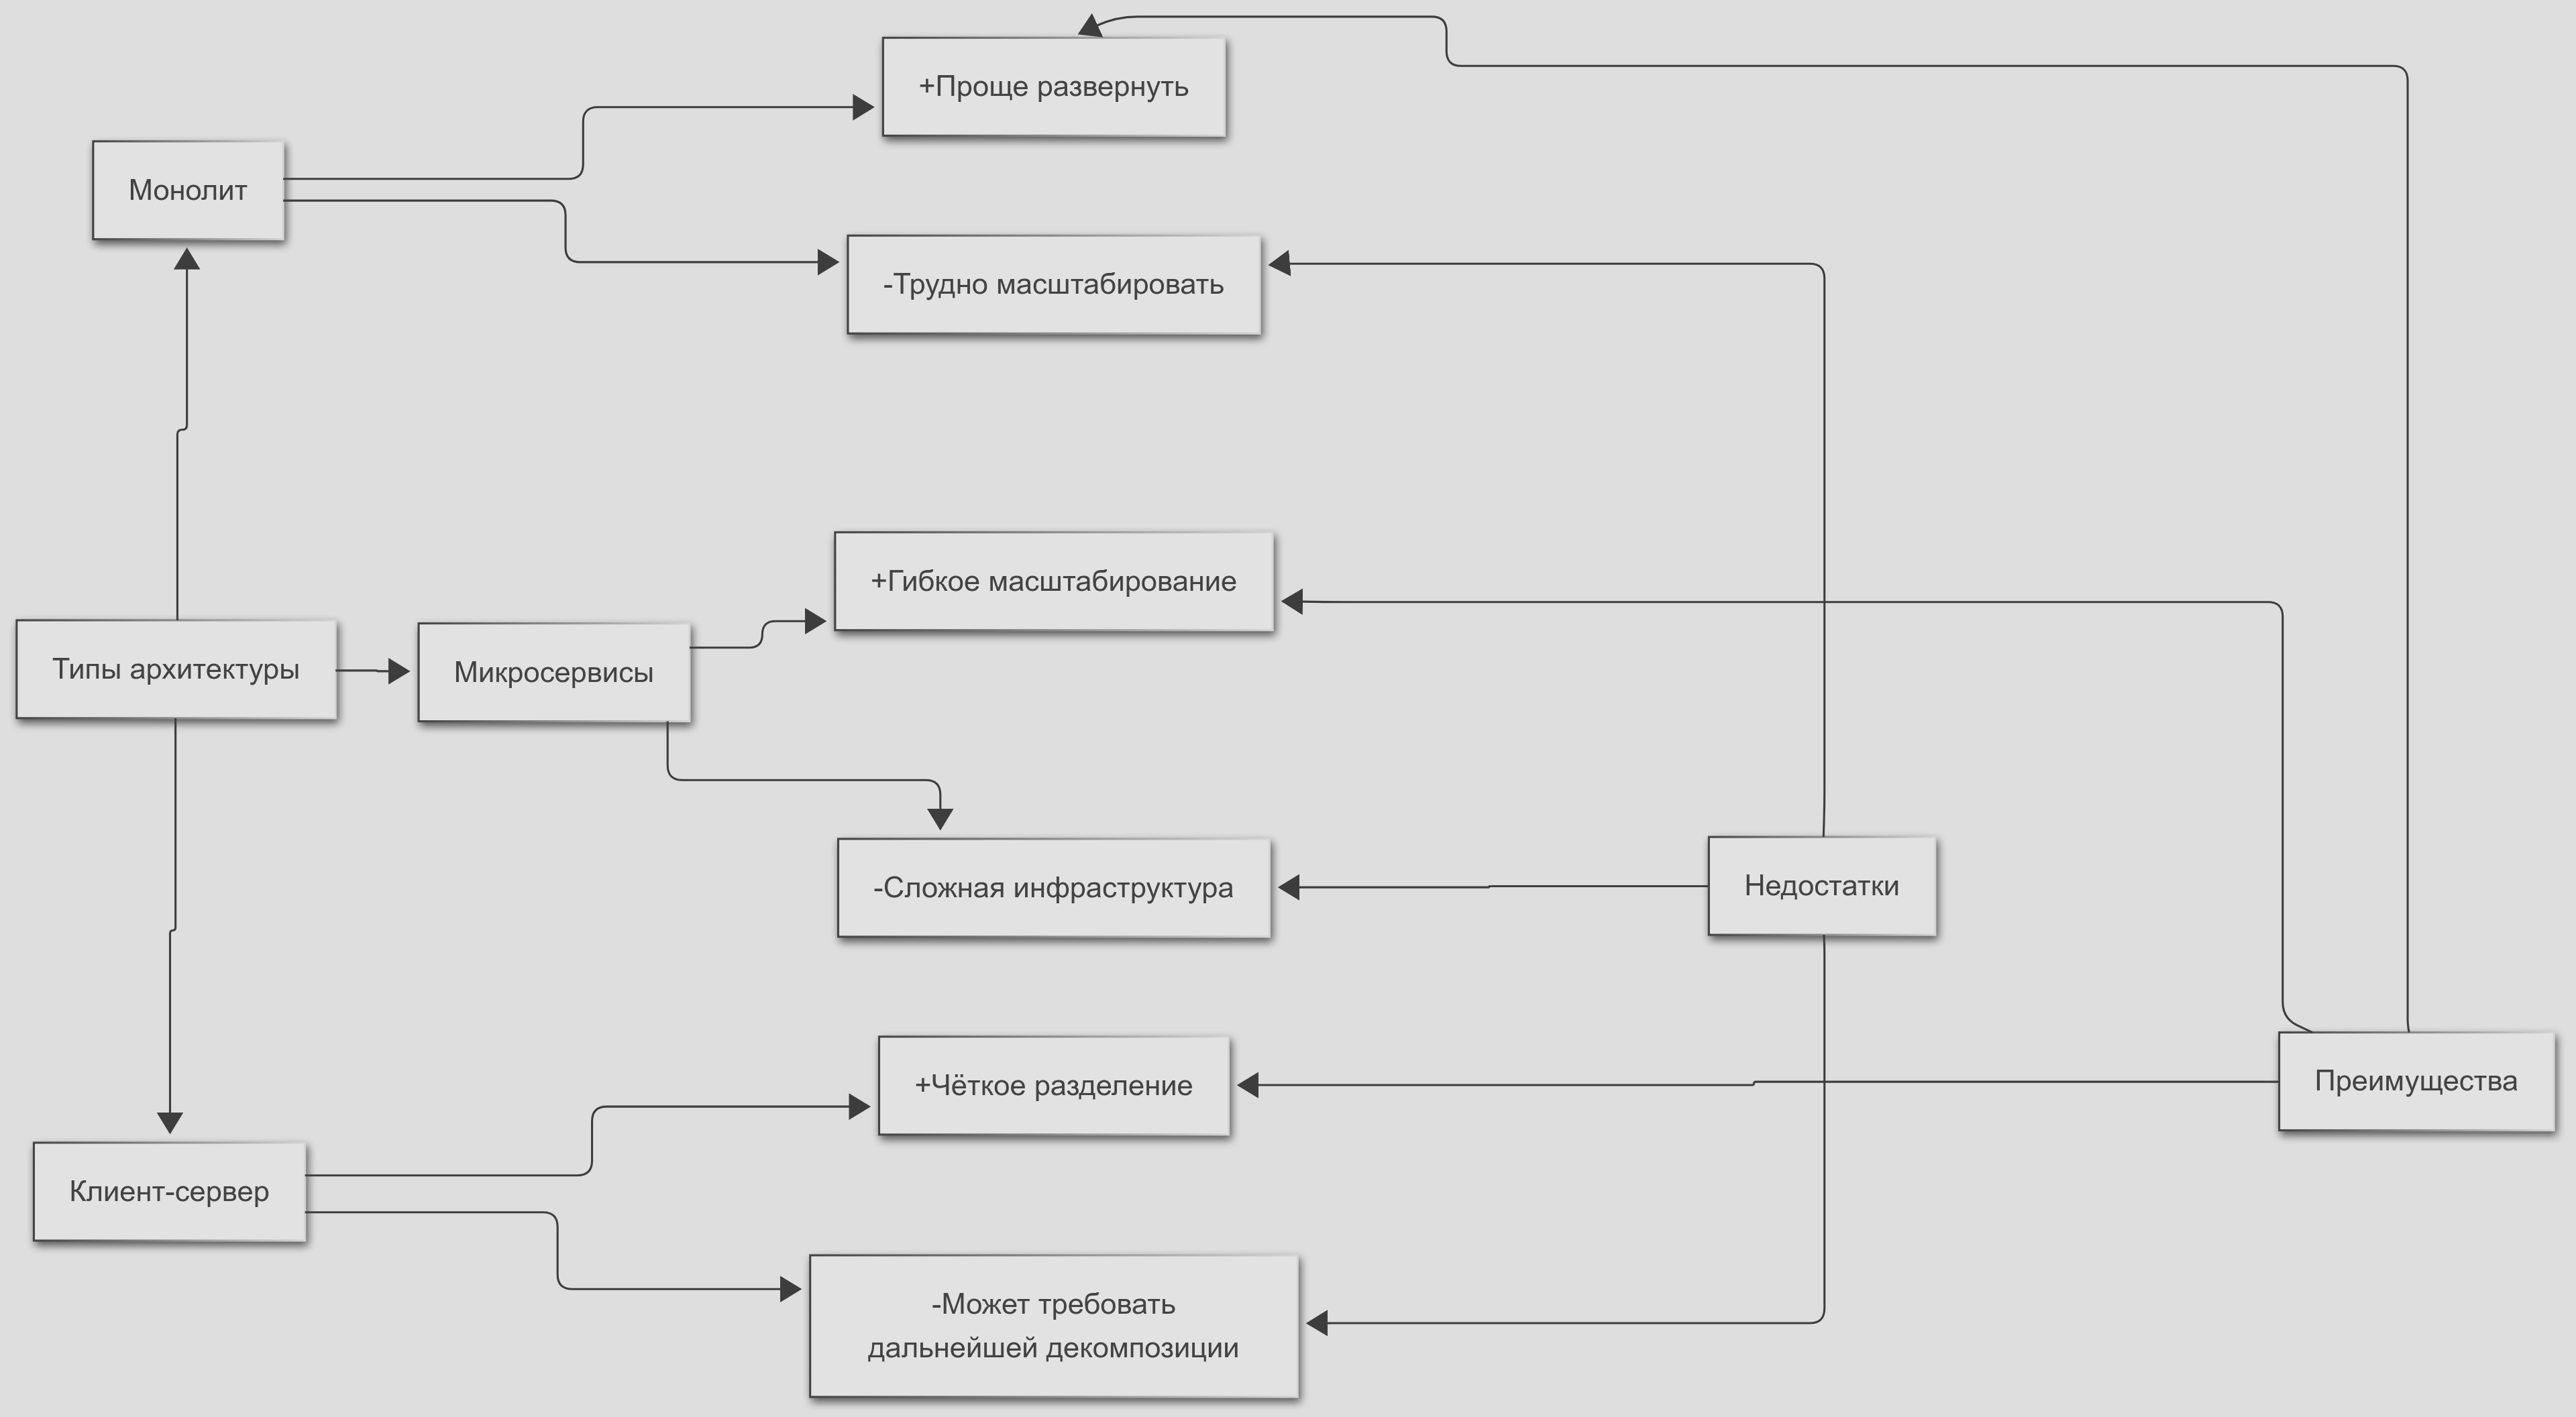
\includegraphics[width=0.9\textwidth]{picture/diploma_architecture_prototypes.png}
    \caption{Типы архитектуры с их основными преимуществами и недостатками}
    \label{architecture_prototypes}
\end{figure}
При разработке платформы для интерактивного формирования запросов важен выбор архитектуры приложения. Рассмотрим основные варианты – монолитная, микросервисная, клиент-серверная – и их плюсы/минусы применительно к нашей задаче описанные на рисунке \ref{architecture_prototypes}.

Монолитная архитектура. Монолитом называют цельное приложение, где все компоненты (интерфейс, логика, обработка данных, модель ИИ) развернуты как единое целое. Такой подход традиционно проще на начальных этапах: вся логика сосредоточена в одном кодовом базе, изменения вносятся централизованно. Преимущества: высокая скорость разработки и простота деплоя – достаточно собрать и развернуть один исполняемый файл или контейнер\cite{atlassian:microservices}. Отладка и тестирование тоже упрощены: легче отследить выполнение запроса от интерфейса до базы, когда всё в одном процессе\cite{atlassian:microservices}.  Производительность зачастую выше, так как компоненты обращаются друг к другу напрямую, без сетевых задержек – одна функция может вызывать другую в памяти. Недостатки: по мере роста проекта монолит может разрастись и стать трудным в поддержке. Малейшее изменение требует пересборки и перезагрузки всего приложения\cite{atlassian:microservices}. Масштабирование осложняется – нельзя увеличить ресурсы только для части системы, например для модуля ИИ, не масштабируя остальное. Ограничена гибкость технологий: если фронтенд, как и бэкенд,  интегрирован в монолит, они жёстко связаны, и переход на другую технологию потребует переписывания значительной части монолита. Также ошибка в одном модуле способна обрушить всё приложение (низкая отказоустойчивость)\cite{atlassian:microservices}. В современных условиях, монолитная архитектура подходит для прототипа или небольшого проекта с ограниченной нагрузкой и командой, когда важны быстрота реализации и простота. Но если платформа будет расширяться (новые модули, большое число пользователей), монолит может стать узким местом.

Микросервисная архитектура. В микросервисном подходе приложение разбивается на ряд независимых сервисов, каждый отвечает за свою функцию (например, отдельный сервис для генерации prompt с помощью ML-модели, отдельный – для управления пользователями и базой данных, отдельный – для фронтенда). Эти сервисы общаются через четко определённые API. Преимущества: гибкость и масштабируемость. Каждый микросервис можно разрабатывать, развёртывать и масштабировать независимо\cite{atlassian:microservices}. Например, если модуль улучшения запросов на основе PyTorch-модели требует много ресурсов, его можно вынести на отдельный сервер(ы) и масштабировать горизонтально при росте нагрузки, не трогая при этом остальные части системы. Обновление одного сервиса не требует останавливать всю платформу – можно выкатить новую версию микросервиса, пока другие работают. Команды разработчиков могут параллельно трудиться над разными сервисами, выбирая оптимальные технологии под задачу (один сервис на Python, другой, скажем, на Node.js, если это оправдано)\cite{atlassian:microservices}. Это ускоряет выпуск новых функций и повышает надёжность: сбой одного микросервиса не обязательно выведет из строя всю систему, остальные будут функционировать. Ключевые плюсы: агильность, независимый деплой, технологическая свобода, высокая отказоустойчивость\cite{atlassian:microservices}. Недостатки: усложняется инфраструктура. Появляется сеть сервисов – нужно настроить их взаимодействие, сервис-дискавери, балансировку, мониторинг каждого компонента\cite{atlassian:microservices}. . Отладка затрудняется: запрос пользователя может пройти через цепочку сервисов, и проследить его путь сложнее (нужна распределённая система логирования). Также микросервисы часто приводят к инфраструктурным оверхедам: каждый сервис требует контейнер, свои ресурсы, настройки CI/CD – число артефактов растёт\cite{atlassian:microservices}. Неконтролируемый рост сервисов (development sprawl) может замедлить разработку, если не вводить стандарты и не управлять зависимостями\cite{atlassian:microservices}. Для небольшой команды микросервисы могут оказаться чрезмерно сложными. Таким образом, имеет смысл переходить к микросервисной архитектуре, когда проект дорастает до масштабов, требующих отдельного масштабирования компонентов или работы больших команд параллельно. 

Клиент-серверная архитектура. Фактически, это классический подход для веб-приложений, предполагающий разделение системы на фронтенд (клиент) и бэкенд (сервер). Клиент и сервер общаются по сети (HTTP/REST или WebSocket). По сути, любое современное веб-приложение уже клиент-серверное, но важно подчеркнуть разделение ролей. Преимущества: разделение ответственности (separation of concerns) – UI и бизнес-логика отделены. Это упрощает поддержку, а также это даёт гибкость разработки: фронтенд-разработчики и бэкенд-разработчики могут работать независимо, используя специализированные инструменты для своих частей. Централизация управления на сервере упрощает обновление логики – код модели и оптимизации prompt хранится на сервере, контроль доступа, безопасность – тоже там, а клиент лишь отображает результаты. Как отмечается в литературе, клиент-сервер обеспечивает лучшую управляемость и безопасность за счёт концентрации ресурсов и данных на сервере\cite{kitrum:clientserver},\cite{enjoyalgorithms:clientserver}.


Дополнительно, можно рассмотреть и другие варианты архитектур. Например, Serverless/FaaS – когда отдельные функции (например, улучшение prompt) развёрнуты как безсерверные функции AWS Lambda или аналогов. Это обеспечивает автомасштабирование и оплату «по факту использования». Однако интеграция долгоживущих моделей в lambdas затруднительна из-за ограничений по времени выполнения и памяти. Многослойная архитектура (трёхуровневая) – где есть ещё слой базы данных, кэширующие прослойки – может применяться при большом числе пользователей и необходимости хранения истории запросов, рейтингов и т.д. Но на концептуальном уровне она схожа с клиент-сервером, просто добавляются инфраструктурные детали.

Резюмируя: для старта платформы интерактивной генерации промптов достаточно архитектуры «клиент сервер». Это разделит front/back, обеспечит удобную разработку и деплой. По мере роста нагрузки или функциональности можно выделять микросервисы – например, вынести генерацию улучшенных запросов в отдельный сервис, который можно масштабировать независимо (например, несколько инстансов с моделью на PyTorch за балансировщиком). Монолитный же вариант уместен только для простейшего прототипа или офлайн-приложения. В современном веб-окружении разделение на фронтенд и бэкенд – де-факто стандарт, обеспечивающий и модульность, и централизованное управление данными\cite{enjoyalgorithms:clientserver}. Модели и подходы для генерации улучшенных запросов

Последний аспект – как именно реализовать автоматическое улучшение промптов средствами NLP/ML в рамках выбранного технологического стека. Существуют разные подходы один из которых представлен на рисунке \ref{prompt_enchancement}: от простых правил и шаблонов до обучения нейросетей, которые переписывают запросы пользователя в оптимизированной форме. Рассмотрим несколько вариантов:

\begin{figure}[htbp]
    \centering
    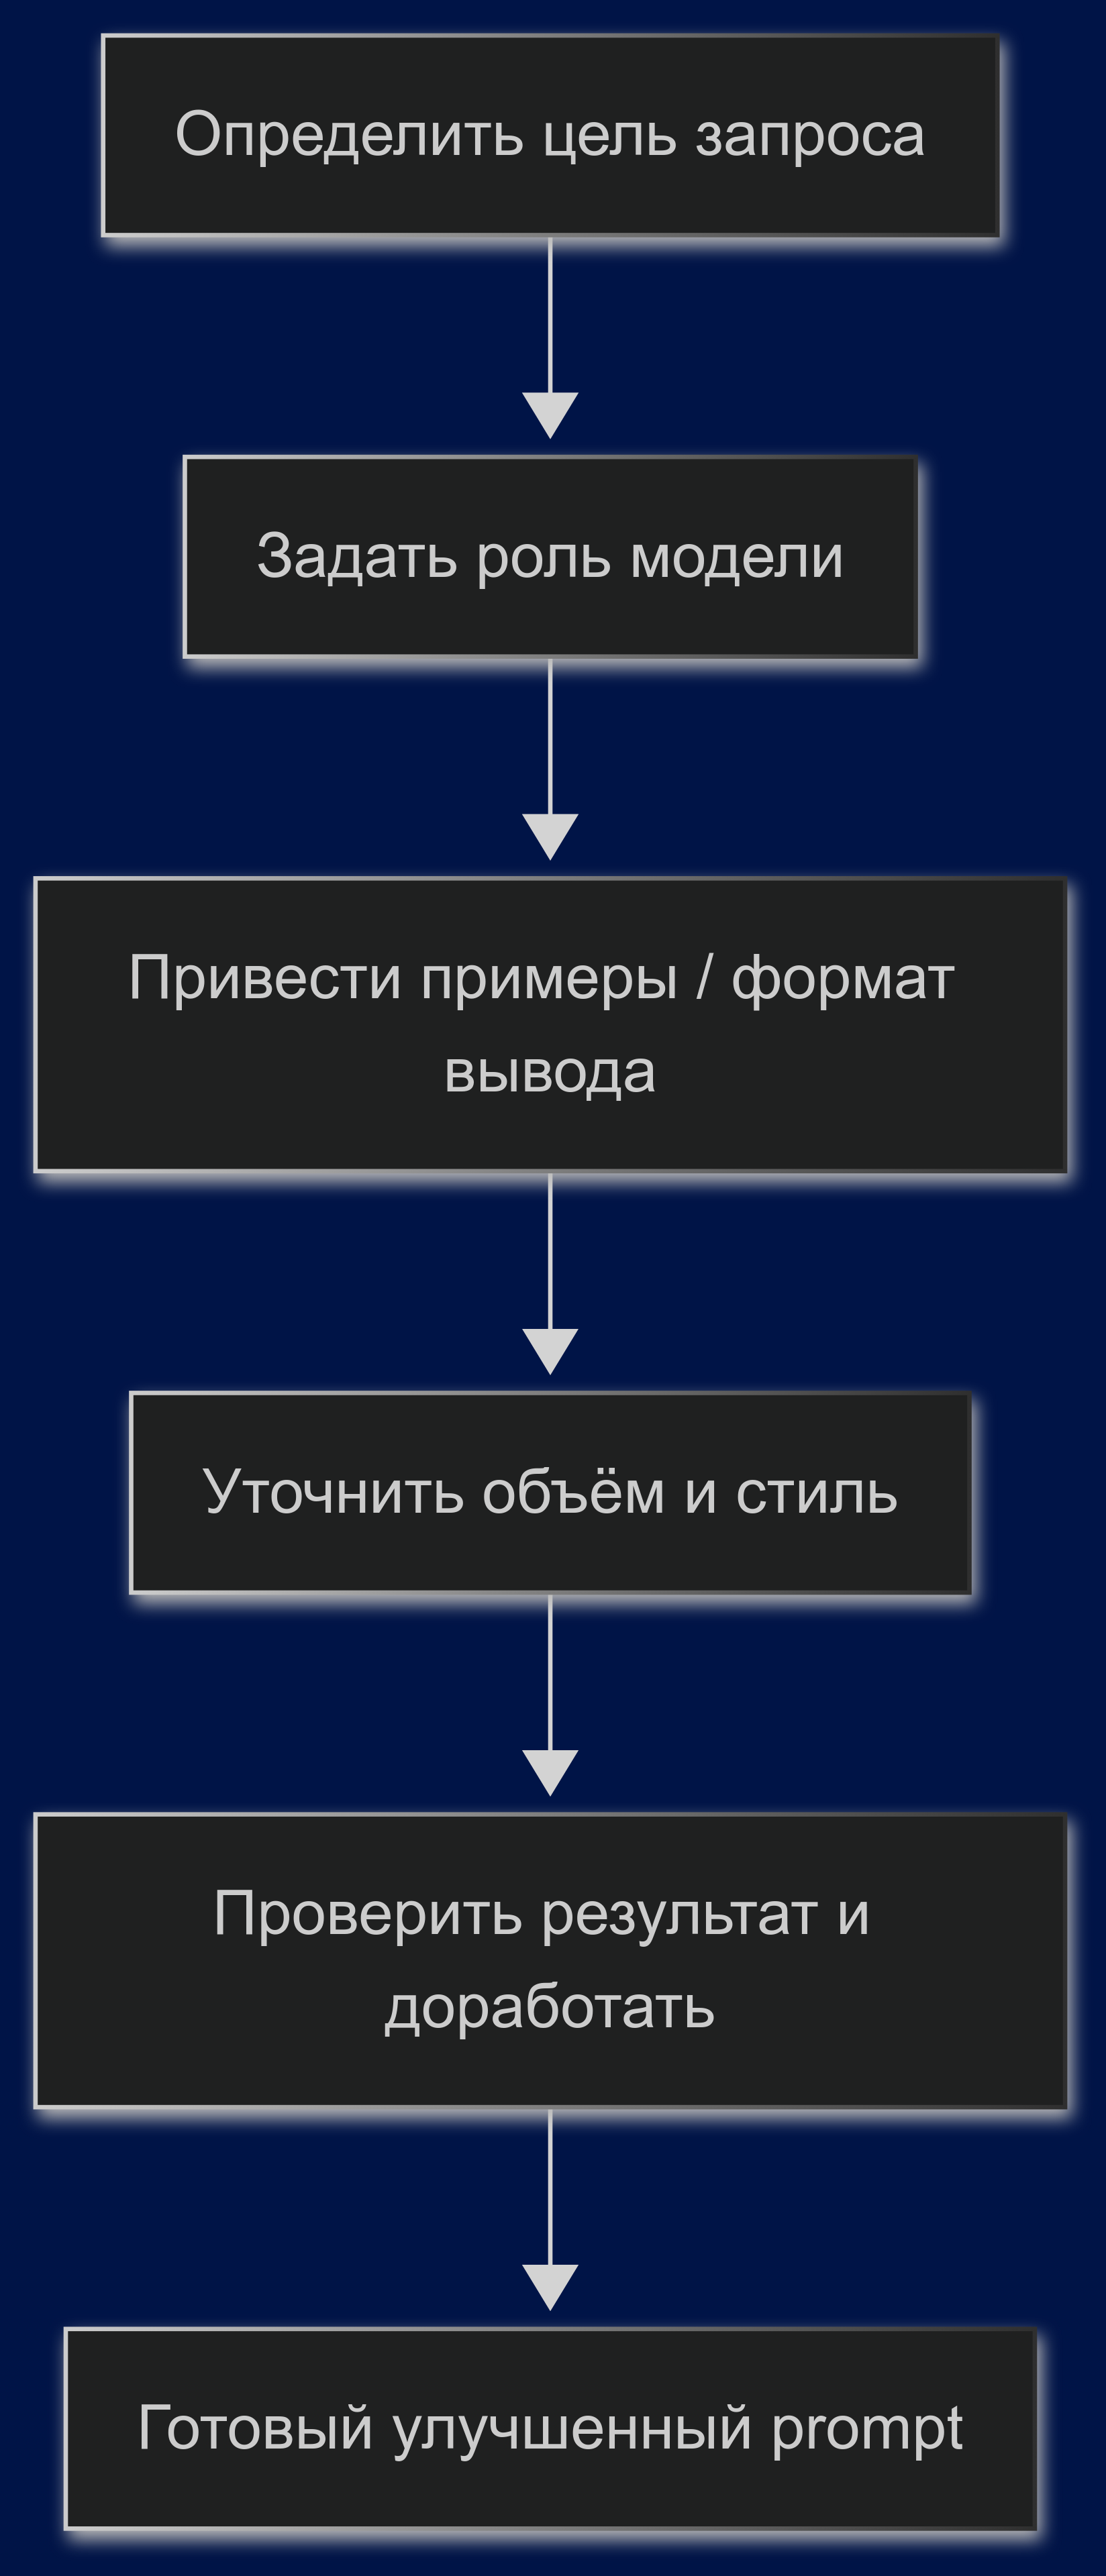
\includegraphics[height=0.7\textwidth]{picture/diploma_prompt_enchantement.png}
    \caption{Алгоритм улучшения запроса}
    \label{prompt_enchancement}
\end{figure}

\begin{enumerate}[label=\arabic*]

\item Правила и лингвистические методы (NLP без глубокого обучения). Используя NLTK, можно выполнить базовый лингвистический анализ prompt’а: токенизация, определение частей речи, разбор предложения. Это пригодится для реализации простых эвристик улучшения. Например, можно проверить длину запроса – если он слишком короткий или состоит из одного-двух слов, платформа может подсказать пользователю добавить деталей (либо автоматически сделать запрос уточняющим вопросом). NLTK также предоставляет тезаурусы (например, WordNet) – их можно использовать, чтобы обогащать текст синонимами или более точными терминами. Предположим, пользователь ввёл: «расскажи про кошек». Автоматически можно заменить расплывчатое «расскажи» на более конкретное «дай обзор повадок домашних кошек, включая.» и т.д. – часть данных (например, список аспектов ухода за кошками) можно хранить как шаблоны (в Pandas DataFrame или БД) и подставлять по теме. Такие улучшения можно делать на основе ключевых слов: распознав слово «кошки», подставить часто запрашиваемые связанные детали (питание, здоровье, породы). Это похоже на экспертную систему: по теме запроса добавляются уточняющие фразы. Плюсы: простота реализации, полная контроль и интерпретируемость – мы точно знаем, что меняем в запросе. Минусы: сложно масштабируется на все темы – нужен словарь или база знаний, иначе ограничится несколькими предметными областями. Кроме того, без понимания контекста можно ошибиться – синоним может не подойти точно по смыслу. Однако для базовых улучшений (например, добавление в конец просьбы «дай ответ списком шагов» или «форматируй ответ в JSON», если пользователь отметил нужный формат) – правила подходят отлично. Мы можем реализовать набор опций: пользователь на фронтенде флажками выбирает «Detailed response», «Bulleted format», «Include examples» – а на бэкенде простой код на Python/NLTK добавляет соответствующие строки к prompt’у. Такая система не обучается, но повышает качество запросов по заранее заданным шаблонам.

\item Использование предобученных языковых моделей (LLM) для перефразирования. Более продвинутый путь – привлечь саму мощь LLM для улучшения prompt. Например, интегрировать вызов OpenAI GPT-4 API: передав в него что-то вроде «Преврати следующий запрос пользователя в максимально подробный и ясный prompt для ИИ: '<пользовательский запрос>'». GPT-4 способен сам сгенерировать улучшенный вариант, опираясь на свой опыт. В этом подходе мы как бы вкладываем один слой ИИ внутрь нашего приложения – мета-ИИ, который помогает обращаться к ИИ. Кстати, именно так работают плагины вроде AISEO и PromptPerfect, только используя API-ключи и, возможно, собственные модели. Плюсы: качество – современные LLM близки к уровню человека в составлении инструкций\cite{restack:advprompt}. Исследования показывают, что большие модели способны быть «prompt engineer»-ами на уровне человека\cite{arxiv:2211.01910}. Метод, известный как Automatic Prompt Engineer (APE), поручает модели генерировать несколько вариантов инструкций и тестировать их, выбирая лучший\cite{restack:advprompt}. Это можно реализовать и онлайн: например, сгенерировать 3 версии запроса, прогнать через целевую модель (или оценить вероятности токенов) и выбрать наиболее результативный. GPT-4, конечно, ресурсозатратен, но дает отличные перефразирования. Минусы: зависимость от внешнего API (если используем его) или высокая нагрузка на сервер (если разворачивать свой LLM). Также может быть непредсказуемость – нужно тщательно настроить системные подсказки, чтобы модель-улучшатель не исказила смысл. Но в контролируемых рамках (с фиксированным prompt-шаблоном для улучшения) это работает.


\item Классические ML-алгоритмы. Можно подойти и с точки зрения обучения более простых моделей: например, классификатор, определяющий, каких элементов не хватает в prompt’е. Используя Pandas, можно проанализировать множество запросов (например, от пользователей платформы), отметить случаи, где не указана роль, или не задан формат ответа. Затем обучить модель (даже решающее дерево или логистическую регрессию) предсказывать, что нужно добавить. Однако, такие решения уступают по гибкости нейросетям. Поэтому чаще либо правила, либо уже end-to-end генерация текстов.

\item Специализированные алгоритмы оптимизации промптов. В научных публикациях появляются методы, позволяющие улучшать запросы автоматически. Помимо упомянутого APE (поиска лучшего инструктажа), есть подход Meta-Prompting – когда модель обучается сама придумывать эффективные инструкции без внешних данных.Также существуют методы с участием пользователя: интерактивные, когда система генерирует несколько вариантов перефразированного запроса, и пользователь выбирает лучший (это своего рода обучение с подкреплением от пользователя). Можно реализовать интерфейс, где после автоматического улучшения prompt показывается пользователю: «Вот так лучше? [Да/Нет]», и если нет – дать другой вариант. Получая обратную связь, система могла бы обучаться (например, методом reinforcement learning, настраивая веса модели-генератора). Это более сложная схема, но она приближает работу платформы к совместному творчеству с пользователем, а не просто «чёрному ящику».

\end{enumerate}

Важно также учесть время отклика. Улучшение запроса должно происходить быстро (идеально < 1-2 секунд), чтобы интерфейс оставался отзывчивым. Правила NLP выполняются миллисекунды, а вот вызов большой модели – может занять секунды. Поэтому, возможно, нужно кешировать результаты или использовать облегченные модели. Один из компромиссов – делать улучшение по требованию: например, если пользователь явно нажал кнопку «Enhance». Если же пользователь уже изначально дал хороший подробный запрос, система может и не тратить время (определив метрикой, что prompt достаточно длинный или содержит все элементы). Здесь Pandas пригодится для хранения статистики: например, средняя длина prompt’ов, какие улучшения чаще всего применяются – это поможет тонко настроить, когда включать ту или иную модель.

Подытоживая, возможные модели для улучшения запросов лежат на спектре от полностью ручных (статические шаблоны, правила) до полностью автоматических (нейросети, генерирующие идеальный prompt). На практике часто эффективна гибридная система: базовые вещи (формат, вежливость, явные ошибки) чинит простая логика, а тонкие стилистические или содержательные улучшения доверяются нейросети. Такой подход даст и качество, и предсказуемость.


\subsection{Вывод}
В результате проведенного анализа можно сделать следующие выводы: сочетание хорошо продуманных правил и современных моделей позволит создать платформу, где пользователь в интерактивном режиме получает подсказки и автоматическую помощь в формулировании запросов к ИИ. Применяя описанные методы детализации prompt’ов и опираясь на опыт существующих систем, можно значительно повысить качество взаимодействия с языковыми и генеративными нейросетями, делая их более доступными и эффективными инструментами. Каждый компонент стека – от Vue-интерфейса до Docker-оркестрации – играет роль в этой системе, обеспечивая удобство, масштабируемость и воспроизводимость решения. Таким образом, интегрируя технические и методологические аспекты, мы получаем мощную платформу для интерактивного prompt engineering, объединяющую лучшее из мира человеко-машинного сотрудничества.